%%%%%%%%%%%%%%%%%%%%%%%%%%%%%%%%%%%%%%%%%%%%%%%%%%%%%%%%%%%%%%%%%%%%%%
% Lớp 10 | Bất phương trình bậc 2 một ẩn | Dấu của tam thức bậc 2
% Dạng 0D7?1-1: Xác định tam thức bậc 2
% Số câu: 15  (sinh tự động bởi tach_cau.py; từ nay thầy sửa trực tiếp file này)
%%%%%%%%%%%%%%%%%%%%%%%%%%%%%%%%%%%%%%%%%%%%%%%%%%%%%%%%%%%%%%%%%%%%%%

%%%%%%%%%%%%%%%% TRẮC NGHIỆM 4 PHƯƠNG ÁN %%%%%%%%%%%%%%%%

% nguồn: MaHoaNH_TracNghiem_Lop10
\begin{ex}%[0D7N1-1]%[ma:2aec2451]
	Cho tam thức bậc hai $f(x)=a x^2+b x+c$  $(c \neq 0)$. Đặt $\Delta=b^2-4a c$. Khẳng định nào sau đây đúng?
	\choice 
		{Nếu $\Delta < 0$ thì $f(x)$ luôn trái dấu  với hệ số $a$, với mọi $x \in \mathbb{R}$}
		{Nếu $\Delta < 0$  thì $f(x)$ luôn cùng dấu với hệ số $b$, với mọi $x \in \mathbb{R}$}
		{Nếu  $\Delta > 0$ thì $f(x)$ luôn cùng dấu với hệ số $a$, với mọi $x \in \mathbb{R}$}
		{\True Nếu $\Delta=0$ thì $f(x)$ luôn cùng dấu với hệ số $a$, với mọi $x \in  \mathbb{R} \setminus\left\{-\dfrac{b}{2a}\right\}$}
	\loigiai{ 
	Theo định lí về dấu của tam thức bậc hai, nếu $\Delta=0$ thì $f(x)$ luôn cùng dấu với hệ số $a$, với mọi $x \in \mathbb{R}  \setminus\left\{-\dfrac{b}{2a}\right\}$.}
\end{ex}

% nguồn: MaHoaNH_TracNghiem_Lop10
\begin{ex}%[0D7N1-1]%[ma:45bbbaee]
	Tìm tất cả các giá trị của tham số $m$ để biểu thức $f(x)=(m-2)x^2+2x-3$ là một tam thức bậc  hai.
	\choice 
		{$m\in \mathbb{R}$} 
		{\True $m\ne  2$}
		{$m  > 2$}
		{$m <  2$}
	\loigiai{ 
		$f(x)=(m-2)x^2+2x-3$ là một tam thức bậc hai khi và chỉ  khi: $m-2\ne 0\Leftrightarrow m\ne 2$.
	} 
\end{ex}

% nguồn: MaHoaNH_TracNghiem_Lop10
\begin{ex}%[0D7N1-1]%[ma:321d4d83]
	Biểu thức nào trong các  biểu thức sau là tam thức bậc hai?
	 \choice
		{$f(x)=2\,023x-2\,022$} 
		{\True  $f(x)=x^2-2\,023x+2\,022$}
		 {$f(x)=\dfrac{2\,023}{x^2}+2\,022x+1$}
		{$f(x)=x^2-\dfrac{2\,023}{x}+2\,022$} 
	 \loigiai{
		Biểu thức $f(x)=x^2-2\,023x+2\,022$ là tam  thức bậc hai.
	 }
\end{ex}

% nguồn: MaHoaNH_TracNghiem_Lop10
\begin{ex}%[0D7N1-1]%[ma:b3f7dee9]
	Tìm tất cả  các giá trị của tham số $m$ để biểu thức $f(x)=\left(m-2\right)x^2+2x-3$ là một tam thức bậc hai.
	\choice 
		{$m\in \mathbb{R}$} 
		{\True $m\ne  2$}
		{$m > 2$} 
		 {$m < 2$}
	 \loigiai{
		Biểu thức $f(x)=\left(m-2\right)x^2+2x-3$ là một tam thức bậc hai khi $m-2\ne 0\Leftrightarrow m\ne  2$.
	} 
\end{ex}

% nguồn: MaHoaNH_TracNghiem_Lop10
\begin{ex}%[0D7N1-1]%[ma:4c4b3015]
	Cho tam thức bậc hai $f(x)=ax^2+b x+c$ $(a \neq 0)$.  Điều kiện để $f(x)>0, \forall x \in \mathbb{R}$ là
	\choice 
		{\True $\heva{&a>0\\&\Delta<0}$} 
		 {$\heva{&a>0\\&\Delta\ge 0}$}
		{$\heva{&a>0\\&\Delta= 0}$} 
		 {$\heva{&a>0\\&\Delta> 0}$}
	 \loigiai{
		 Ta có $f(x)>0, \forall x \in \mathbb{R}\Leftrightarrow\heva{&a>0\\&\Delta<0.} $
	} 
\end{ex}

% nguồn: MaHoaNH_TracNghiem_Lop10
\begin{ex}%[0D7N1-1]%[ma:a99b2bb0]
	Cho $f(x)=ax^2+bx+c$ với $a\ne 0$ và $\Delta=b^2-4ac$. Hãy cho biết dấu của $\Delta$ khi $f(x)$ luôn cùng dấu với hệ số $a$ với  mọi $x\in \mathbb{R}$.
	\choice 
		 {$\Delta > 0$}
		{\True $\Delta < 0$} 
		{$\Delta \le  0$}
		{$\Delta  \ge 0$}
	\loigiai{ 
		 Để $f(x)$ luôn cùng dấu với hệ số $a$ với mọi $x\in \mathbb{R}$ thì $\Delta < 0$.
	} 
\end{ex}

% nguồn: MaHoaNH_TracNghiem_Lop10
\begin{ex}%[0D7N1-1]%[ma:2c9e4cb1]
	Cho tam thức $f(x)=ax^2+bx+c$ với $a\ne 0$ và $\Delta=b^2-4ac$. Ta có  $f(x)\le 0, \; \forall x \in \mathbb{R}$ khi và chỉ khi
	\choice 
		 {$\heva{&a > 0\\&\Delta\le 0}$}
		{$\heva{&a\le 0\\&\Delta < 0}$} 
		{\True $\heva{&a  < 0\\&\Delta\le 0}$}
		 {$\heva{&a < 0\\&\Delta\ge 0}$}
	\loigiai{ 
		Ta có $f(x)\le 0$, $\forall x  \in \mathbb{R}$ khi và chỉ khi $\heva{&a<0\\&\Delta\le0}$.
	} 
\end{ex}

% nguồn: MaHoaNH_TracNghiem_Lop10
\begin{ex}%[0D7N1-1]%[ma:8757403b]
	Nghiệm của tam thức bậc hai $f(x)=x^2-9$  là
	\choice 
		{$x=-3$} 
		 {$x=3$}
		{\True  $\hoac{&{x=3} \\
		 &{x=-3}
		&}$} 
		{$\hoac{&{x=0} \\ 
		&{x=9} 
		 &}$}
	 \loigiai{
		 Ta có $f(x)=0\Leftrightarrow x=\pm 3$.
	} 
\end{ex}

% nguồn: MaHoaNH_TracNghiem_Lop10
\begin{ex}%[0D7N1-1]%[ma:92ee5a90]
	Trong các biểu thức sau, biểu thức  nào là tam thức bậc hai?
	 \choice
		 {\True $f(x)=x^2+3$}
		 {$f(x)=2x+3$}
		 {$f(x)=mx^2+3$}
		 {$f(x)=\sqrt{2x^2+3}$}
	\loigiai{ 
		Tam thức bậc hai là tam thức có dạng  $f(x)=ax^2+bx+c$ với $a \neq 0$.\\
		Phương án $f(x)=x^2+3$ với $a=1$; $b=0$; $c=3$ nên $f(x)=x^2+3$ là tam thức bậc  hai.\\
		 Phương án $f(x)=2x+3$ là nhị thức bậc nhất.\\
		Phương án $f(x)=mx^2+3$ với $a=m$; $b=0$; $c=3$, vì $m$  chưa xác định nên $f(x)=mx^2+3$ không phải là tam thức bậc hai.\\
		Phương án  $f(x)=\sqrt{2x^2+3}$ không có dạng $f(x)=a x^2+bx+c$ nên $f(x)=\sqrt{2x^2+3}$ không phải là tam thức bậc hai.
	 }
\end{ex}

% nguồn: MaHoaNH_TracNghiem_Lop10
\begin{ex}%[0D7N1-1]%[ma:e38ee1c2]
	Bảng xét dấu  sau là của biểu thức nào?
	\begin{center}
		\begin{tikzpicture}
				 \tkzTabInit[nocadre=false,lgt=1.2,espcl=2.5,deltacl=0.6]
					{$x$  /.7,$f (x)$ /.7}{$-\infty$,$1$,$2$,$+\infty$}
				\tkzTabLine{,-,$0$,+,$0$,-} 
			\end{tikzpicture}
	\end{center}
	\choice 
		{\True $f(x)=-x^2+3x-2$} 
		 {$f(x)=x^2-3x+2$}
		 {$f(x)=-x^2-3x+2$}
		{$f(x)=x^2+3x+2$} 
	 \loigiai{
		Dựa vào bảng xét dấu ta thấy  tam thức bậc hai phải chọn có $a < 0$ và có nghiệm là $1$ và $2$.\\
		Vậy  $f(x)=-x^2+3x-2$.
	} 
\end{ex}

% nguồn: MaHoaNH_TracNghiem_Lop10
\begin{ex}%[0D7H1-1]%[ma:30c1d7aa]
	Xét tam thức bậc hai $f(x)=-3x^{2}+2x-1$. Khẳng định nào sau  đây đúng?\\
	\choice 
		{$f(x)>0$,  $\forall x\in \mathbb{R}$}
		{$f(x)\leq 0$, $\forall x\in \mathbb{R}$} 
		{$f(x)\geq 0$, $\forall x\in  \mathbb{R}$}
		 {\True $f(x)<0$, $\forall x\in \mathbb{R}$}
	 \loigiai{
		Xét $f(x)=-3x^{2}+2x-1$.\\ 
		Vì $\Delta'=1-(-3)\cdot(-1)=-2<0$ và $a=-3<0$ nên $f(x)<0$, $\forall x\in \mathbb{R}$.\\ 
	 }
\end{ex}


%%%%%%%%%%%%%%%% ĐÚNG/SAI %%%%%%%%%%%%%%%%

% nguồn: MaHoaNH_DungSai_Lop10
\begin{ex}%[0D7N1-1]%[ma:07843be2]
	Mỗi khẳng  định dưới đây đúng hay sai?
	\choiceTF 
		{\True $f(x)=3x^2+2x-5$  là tam thức bậc hai ẩn $x$}
		{$g(x)=(m-1)x^2+2x+5$, với $m\in\mathbb{R}$, là tam thức bậc hai  ẩn $x$}
		{Tam thức bậc hai $h(x)=-2x^2+x-3$ có hai nghiệm phân  biệt}
		{\True Tam thức bậc hai  $k(x)=4x^2+4x+1$ có nghiệm kép}
	 \loigiai{
		\begin{itemchoice}
			\itemch $f(x)=3x^2+2x-5$ là  tam thức bậc hai ẩn $x$.
			\itemch  $g(x)=(m-1)x^2+2x+5$ là tam thức bậc hai ẩn $x$ khi $m\neq 1$.
			\itemch  Tam thức bậc hai $h(x)=-2x^2+x-3$ có biệt thức $\Delta=1-4\cdot(-2)\cdot(-3)<0$ nên vô nghiệm.
			\itemch Tam thức bậc hai $k(x)=4x^2+4x+1$ có biệt  thức $\Delta'=2^2-4\cdot 1=0$ nên có nghiệm kép.
		\end{itemchoice}
	} 
\end{ex}

% nguồn: MaHoaNH_DungSai_Lop10
\begin{ex}%[0D7N1-1]%[ma:4ac42da9]
	Các mệnh đề sau đúng hay sai? 
	\choiceTF 
		{$3x+7$ là tam thức bậc hai} 
		{\True  $-x^2+3$ là tam thức bậc hai}
		{\True $3x(x-1)$ là tam thức bậc hai} 
		 {$(x-1)(x+1)-x^2$ là tam thức bậc hai}
	 \loigiai{
		\begin{itemchoice}
			\itemch Sai. Vì $3x+7$ không có dạng $ax^2+bx+c$. 
			\itemch Đúng. Vì $-x^2+3$ nó có  dạng $ax^2+bx+c$.
			\itemch Đúng.  Vì $3x(x-1)=3x^2-3x$ là tam thức bậc hai.
			\itemch Sai.  Vì $(x-1)(x+1)-x^2=x^2-1-x^2=1$.
		\end{itemchoice}
	} 
\end{ex}

% nguồn: MaHoaNH_DungSai_Lop10
\begin{ex}%[0D7H1-1]%[ma:a3343b90]
	 Cho tam thức bậc hai $f(x)=-x^2+x+3$.
	\choiceTF 
		{Tam thức bậc hai  $f(x)$ vô nghiệm}
		 {\True Tam thức bậc hai $f(x)$ dương tại $x=2$}
		{Tam thức bậc hai $f(x)$ dương tại $x=-3$} 
		{\True Tam  thức bậc hai $f(x)$ âm tại $x=3$}
	\loigiai{ 
		\begin{itemchoice}
			\itemch Tam thức bậc hai $f(x)=-x^2+x+3$ có biệt thức $\Delta=1-4\cdot(-1)\cdot 3>0$ nên có hai nghiệm  phân biệt.
			\itemch Ta có $f(2)=-2^2+2+3=1>0$ nên $f(x)$ dương tại $x=2$. 
			\itemch Ta có $f(-3)=-(-3)^2-3+3=-9<0$  nên $f(x)$ âm tại $x=-3$.
			\itemch Ta có $f(3)=-3^2+3+3=-3<0$ nên  $f(x)$ âm tại $x=3$.
		\end{itemchoice}
	} 
\end{ex}


%%%%%%%%%%%%%%%% TỰ LUẬN %%%%%%%%%%%%%%%%

% nguồn: MaHoaNH_TuLuan_Lop10
\begin{bt}%[0D7B1-1]%[ma:d7e16238]
	 Tìm tất cả các giá trị của tham số $m$ để bất phương trình $mx^{2}-2(m+1)x+m+3>0$ thỏa mãn với mọi $x\in\mathbb{R}$.
	 \loigiai{
		Xét $mx^{2}-2(m+1)x+m+3>0$. \quad  $(1)$
		\begin{itemize}
			\item Với $m=0$ thì $(1)$ trở thành $-2x+3>0 \Leftrightarrow x<\dfrac{3}{2}$. Suy ra  $m=0$ không thỏa mãn.
			\item Với $m\ne 0$ thì  $(1)$ luôn đúng với mọi $x\in\mathbb{R}$ khi và chỉ khi
			\[\heva{&m>0\\&\Delta'=(m+1)^{2}-m(m+3)<0} \Leftrightarrow \heva{&m>0\\&-m+1<0}  \Leftrightarrow \heva{&m>0\\&m>1} \Leftrightarrow m>1.\]
		\end{itemize}
		Vậy $m>1$ là giá trị  cần tìm.
	 }
\end{bt}
